%%%%%%%%%%%%%%%%%%%%%%%%%%%%%%%%%%%%%%%%%%%%%%%%%%%%%%%%%%%%%%%%%%%%%%%%%%%%%%%
%Objetivo: Caracterizas as Ferramentas de Gerenciamento de Requisição de Mudança
%		   com base nas suas funcionalidades
%Autor: Vagner Clementino <vagnercs@dcc.ufmg.br>
% 		Rodolfo Resende	<rodolfo@dcc.ufmg.br>
%Criação: qua set 28 11:25:03 BRT 2016
%Modificação: Seg Nov  7 14:59:04 BRST 2016
%Revisão: Seg Nov 21 20:51:41 BRST 2016
%%%%%%%%%%%%%%%%%%%%%%%%%%%%%%%%%%%%%%%%%%%%%%%%%%%%%%%%%%%%%%%%%%%%%%%%%%%%%%%
\chapter{Caracterização das Ferramentas de Gerenciamento de Requisição de
	Mudança}
\label{ch:caracterizacao_ferramentas}

\section{Introdução}
\label{sec:caracterizacao_intro}
Quando uma empresa ou um projeto de software de código aberto decide adotar uma
Ferramenta de Gerenciamento de Requisições de Mudança~-~FGRM o desafio é
encontrar aquela que melhor atenda suas necessidades. Um possível fundamento de
seleção é o conjunto de funcionalidades oferecidas pelo sistema. Outros
critérios podem envolver o custo ou o suporte a falhas da ferramenta. De
maneira relacionada, o pesquisador que estuda propostas de melhorias para as
FGRM's pode estar interessado em analisar o conjunto de funções comuns que
caracterizam este tipo de software.

O numero de FGRM's disponíveis atualmente é bastante elevado. Em uma inspeção
inicial, verificamos a existência de mais de 50 ferramentas fornecidas
comercialmente ou em código
aberto~\footnote{\url{https://en.wikipedia.org/wiki/Comparison_of_issue-tracking_systems}}.
Apesar das diversas opções disponíveis, ao bem do nosso conhecimento,
desconhecemos estudos que avaliem sistematicamente as funcionalidades oferecidas
por este tipo de ferramenta a fim de compará-las. Entendemos que a partir de um
conjunto compartilhado de funções/comportamento seja possível caracterizar as
FGRM's, ao mesmo tempo possibilita avaliar a contribuição de novas
funcionalidades propostas na literatura, conforme discutido no
Capítulo~\ref{ch:mapeamento-sistematico}. Para alcançarmos este objetivo,
realizamos um estudo exploratório visando determinar as principais
funcionalidades presentes nas FGRM's. Um estudo exploratório está preocupado com
a análise do objeto em sua configuração natural e deixando que as descobertas
surjam da própria observação~\cite{wohlin2012experimentation}. Neste tipo de
estudo nenhuma hipótese é previamente definida.

O trabalho descrito neste capítulo consistiu na leitura da documentação
disponível na Internet de algumas FGRM's de modo a sistematizar as
funcionalidades oferecidas por cada ferramenta.  As funções foram coletadas e
organizadas utilizando a técnica de Cartões de Classificação (Sorting
Cards)~\cite{5070993, rugg2005sorting}. Devido ao alto volume de ferramentas
disponíveis e ao esforço necessário para analisar a documentação de todas elas,
optamos por realizar este estudo com um conjunto mínimo escolhido com a ajuda de
profissionais envolvidos em manutenção de software. Através de um levantamento
(survey) onde os profissionais responderam dentre as ferramentas apresentadas
quais eram as mais representativas dentro do domínio de aplicação das FGRM's. A
representatividade neste contexto não está no número de projetos que utiliza
determinada ferramenta, mas pelas caraterísticas que determinado software possui
que o torna diferenciável dentro do seu domínio.

Este capítulo está organizado da seguinte forma: na
Seção~\ref{sec:objetivo_do_capítulo} discutimos os objetos deste capítulo; na
Seção~\ref{sec:metodologia} apresentamos o método utilizado na condução do
estudo, em especial a técnica de Cartões de Ordenação e o levantamento realizado
com os profissionais para escolher as ferramenta do estudo.

\section{Objetivo do Capítulo}
\label{sec:objetivo_do_capítulo}

O objetivo inicial deste capítulo é apresentar e discutir as principais
funcionalidades das FGRM's que dão suporte ao desenvolvimento e manutenção de
software. Tomando como ponto de partida um conjunto de sistemas definidos como
os mais relevantes por profissionais envolvidos em manutenção e desenvolvimento
de software. Em um segundo momento, o foco foi caracterizar este tipo de
ferramenta tomando como base as funcionalidades oferecidas pelos softwares.
Conforme já exposto, a literatura em Manutenção de Software apresenta diferentes
nomenclaturas para este tipo de ferramenta (Sistema de Controle de Defeito~-~Bug
Tracking Systems, Sistema de Gerenciamento da Requisição~-~Request Management
System, Sistemas de Controle de Demandas (SCD)~-~Issue Tracking Systems), sem,
contudo, se preocupar em diferenciá-las.

Acreditamos que o resultado deste estudo permitirá compreender melhor este tipo
de software tomando como base o conjunto de funções que eles oferecem aos seus
usuários. Também será possível propor novas funcionalidades ou melhorias das
existentes tendo em vista a possibilidade de determinar o conjunto mínimo de
comportamentos deste tipo de ferramenta. Uma outra contribuição é a criação de
uma taxonomia com base nas funcionalidades oferecidas.

\section{Metodologia}
\label{sec:metodologia}

A fim de determinarmos o conjunto das principais funcionalidades das FGRM's que
dão suporte à manutenção e desenvolvimento de software realizamos um estudo
exploratório dividido em três etapas que estão listadas a seguir. O resultado
obtido em etapa foi utilizado para subsidiar as atividades do etapa posterior.
O início de uma nova fase do trabalho era precedido de uma avaliação geral afim
de verificar possíveis inconsistências e avaliação das lições aprendidas.

\begin{enumerate}[(i)]
	\item Seleção das Ferramentas
	\item Inspeção da Documentação
	\item Agrupamento das Funcionalidades
\end{enumerate}

\subsection{Seleção das Ferramentas}
\label{subsec:selecao-ferramentas}

A primeira etapa consistiu da definição das ferramentas que seriam utilizadas no
estudo. A partir de uma pesquisa na Internet obtivemos um conjunto inicial de 50
ferramentas~\footnote{\url{https://en.wikipedia.org/wiki/Comparison_of_issue-tracking_systems}}
que podem ser visualizadas no Anexo~\ref{ch:app-lista-fgrm}. Devido ao esforço
necessário e a dificuldade de realizar a análise em cada uma daquelas
ferramentas, optamos por escolher um subconjunto de sistemas que fossem mais
representativos, tomando como base a opinião de profissionais envolvidos em
manutenção e desenvolvimento de software. A representatividade neste caso
corresponde a opinião do profissional sobre notoriedade que a ferramenta possui
dentro do seu domínio de aplicação em comparação com as demais que lhe foram
apresentadas ou outras do qual tenha prévio conhecimento.

A opinião dos profissionais foi obtida mediante a realização de uma pesquisa
(survey~\cite{wohlin2012experimentation}) realizada com o uso de um formulário
eletrônico. O formulário foi estruturado em duas partes principais: a formação
de base do participante (background) e a avaliação das ferramentas. Na primeira
parte estávamos interessados em conhecer as características do respondente. Esta
informação é relevante tendo em vista que, como descreveremos a seguir, o
questionário foi replicado em três grupos distintos de profissionais. Neste
sentido, foi possível realizar análises sobre como é formado cada um dos grupos
que participaram deste estudo. Na segunda parte da pesquisa apresentamos as
ferramentas e foi solicitado aos participantes que avaliassem a relevância de
cada uma delas através de questões de múltipla escolha. As opções de respostas
foram estruturadas em escala do tipo Likert~\cite{robbins2011plotting}.

Antes da efetiva aplicação do questionário no público-alvo do estudo, o
documento foi validado em um processo de três etapas. Na primeira parte foi
solicitado a dois pesquisadores experientes da área de Engenharia de Software
que avaliassem o formulário. A partir das sugestões obtidas dos pesquisadores
foram realizadas adequações no documento. Após as alteração uma nova versão do
formulário foi enviada para dois profissionais envolvidos diretamente em
manutenção de software. O critério utilizado para seleção dos profissionais foi
o tempo dedicado à tarefa de manter software, que no caso dos desenvolvedores
escolhidos era em média de 10 anos. O formulário foi modificado com as sugestões
dos profissionais finalizando a segunda etapa de validação. A última etapa
consistiu na realização de um piloto com dez profissionais envolvidos em
manutenção de uma empresa pública de informática. Os profissionais tiveram que
preencher o questionário, contudo, foram adicionadas questões as quais era
possível inserir sugestões de melhoria. O resultado deste processo de validação
é o questionário presente no Anexo~\ref{ch:app-form-selecao-ferramentas}. Como o
público-alvo do questionário poderia incluir desenvolvedores de diferentes
nacionalidades foi construído em uma versão em língua inglesa do formulário.

A população de interesse deste levantamento é o conjunto de profissionais
envolvidos em manutenção de software. Naturalmente é difícil definir o tamanho e
características desta população de modo a mensurar uma amostra significativa.
Neste sentido, visando minimizar enviesamento deste estudo, o questionário
foi replicado em três grupos:

\begin{description}
	\item[Grupo 01:] Profissionais de empresa pública e privada de
			desenvolvimento e manutenção de software.
	\item[Grupo 02:] Profissionais que contribuem em projetos de
		código aberto
	\item[Grupo 03:] Profissionais que participam de grupos de
		interesse sobre desenvolvimento e manutenção de software em uma rede
		social profissional (LinkedIn) ou aqueles que participam de discussão
		sobre este assunto em uma rede social (Stack Overflow).
\end{description}

Os participantes que compõe cada grupo foram escolhidos conforme critérios que
são detalhados no Capítulo~\ref{ch:pesquisa-profissionais}. A reutilização desta
base de desenvolvedores se deu por conta de ambos os estudos compartilharem a
mesma população de interesse, podendo neste caso compartilhar a mesma amostra.
Ademais, como o questionário descrito nesta seção foi realizado antes daquele
contido no Capítulo~\ref{ch:pesquisa-profissionais}, as lições aprendidas no
primeiro serviram para melhorar o processo de desenho e execução do segundo.

Com base nos dados obtidos da pesquisa com os profissionais, as FGRM's foram
classificadas como \textit{''ferramentas''} e \textit{''serviços da internet''}.
O primeiro grupo representa os softwares que são capazes de serem implantados na
infraestrutura do seu cliente e permite algum grau de personalização de pelo
menos um dos componentes, como por exemplo, o banco de dados utilizado. No
segundo grupo estão os software que ofertam a gerência das RM's mediante uma
arquitetura do tipo Software como Serviço (Software as
Service)~\cite{fox2013engineering}, onde certos tipos de alterações no
comportamento do software são mais restritas. Acreditamos que ao escolher
ferramentas dos dois tipos descritos anteriormente iremos cobrir uma grande
parte do domínio de aplicação das FGRM's. Optamos por escolher ~\textit{06
	ferramentas} para o estudo, sendo três de cada um dos grupos. Neste sentido,
foram escolhidas as três ferramentas mais relevantes para cada grupo com base
nos dados da pesquisa com os profissionais.

Para seleção das ferramentas utilizados a formula apresentada na
Equação~\ref{eq:escolha_ferramenta}.  Atribuímos a métrica $r_i$ que representa
a relevância de determinada ferramenta $f_i$. A métrica é calculada somando a
frequência de cada um dos graus de relevância apresentado na
Tabela~\ref{tab:graus_relevancia} multiplicado pela pelo grau de relevância
descrito na mesma tabela.

\begin{equation}
\label{eq:escolha_ferramenta}
r_i = \sum_{i=1}^{n} f_i \times w_j
\end{equation}

A documentação de algumas ferramentas, em especial aquelas que adotam uma
arquitetura cliente/servidor e necessitam de um certo grau de administração,
dividem as funcionalidades do software entre aquelas com foco no usuário final e
administradores. Nestes casos optamos por coletar as funcionalidades cujo o foco
seja o usuário da FGRM, tendo em vista que eles, profissionais devotadas às
atividade de manutenção de software, estarem entre o público-alvo desta
dissertação.

\begin{table}[htb]
\centering
	\resizebox{0.6\linewidth}{!}{%
\begin{tabular}{|clc|}
\hline
\textbf{$j$} & \textbf{Grau de Relevância} & \textbf{Peso($w_j$)} \\ \hline
1 & Não conheço a ferramenta & 1 \\
2 & Nada relevante & 2 \\
3 & Pouco relevante & 3 \\
4 & Pouco relevante & 4 \\
5 & Muito relevante & 5 \\ \hline
\end{tabular}%
}
\caption{Graus de Relevância}
\label{tab:graus_relevancia}
\end{table}


\subsection{Inspeção da Documentação}
\label{subsec:inspecao_doumentacao}

Nesta etapa do trabalho realizamos a leitura do material disponível na Internet
para cada uma das ferramentas que foram selecionadas na etapa anterior. Entre
estes materiais utilizamos manuais do usuário e do desenvolvedor e notas de
lançamento. Para cada uma das FGRM's optamos por estudar a última versão estável
do software a fim de analisarmos o que há de mais novo disponível aos usuários.
A Tabela~\ref{tab:fgrm-docs} apresenta as ferramentas analisadas e o elo de
ligação para cada documentação utilizada neste estudo. Para aquelas ferramentas
que apresentam documentação em mais de um idioma optamos sempre por utilizar
aquela escrita em inglês por entendermos ser a que esteja mais atualizada.

\begin{table}[htpb]
\centering
\resizebox{\textwidth}{!}{%
\begin{tabular}{|l|l|}
\hline
\multicolumn{1}{|c|}{\textbf{Nome da Ferramenta}} & \multicolumn{1}{c|}{\textbf{Elo de Ligação}} \\ \hline
Bugzilla & \url{https://www.bugzilla.org/features/} \\
Github Issue Tracking System & \url{https://github.com/blog/411-github-issue-tracker} \\
Github Issue Tracking System & \url{https://github.com/features} \\
Github Issue Tracking System & \url{https://guides.github.com/features/issues/} \\
Gitlab Issue Tracking System & \url{http://docs.gitlab.com/ce/user/project/labels.html} \\
Gitlab Issue Tracking System & \url{https://about.gitlab.com/2016/08/22/announcing-the-gitlab-issue-board/} \\
Gitlab Issue Tracking System & \url{https://about.gitlab.com/solutions/issueboard/} \\
Gitlab Issue Tracking System & \url{https://docs.gitlab.com/ee/user/project/description\_templates.html} \\
Gitlab Issue Tracking System & \url{https://docs.gitlab.com/ee/user/project/issues/automatic\_issue\_closing.html} \\
Gitlab Issue Tracking System & \url{https://docs.gitlab.com/ee/workflow/issue\_weight.html} \\
Gitlab Issue Tracking System & \url{https://docs.gitlab.com/ee/workflow/milestones.html} \\
Gitlab Issue Tracking System & \url{https://docs.gitlab.com/ee/workflow/time\_tracking.html} \\
JIRA & \url{https://br.atlassian.com/software/jira/features} \\
MantisBT & \url{https://www.mantisbt.org/wiki/doku.php/mantisbt:features} \\
Redmine & \url{http://www.redmine.org/projects/redmine/wiki/Features} \\ \hline
\end{tabular}%
}
\caption{Documentações utilizadas no processo de coleta de dados.}
\label{tab:fgrm-docs}
\end{table}

Os dados obtidos da leitura do material disponíveis para cada ferramenta foram
sistematizados por meio de técnica denominada \textit{Cartões de
	Classificação~-~Sorting Cards}. Cartões de Classificação é um técnica de
elicitação de conhecimento, de baixo custo e com foco no usuário, largamente
utilizada em arquitetura informacional para criar modelos mentais e derivar
taxonomias da entrada utilizada~\cite{just2008towards}. Ela envolve a
categorização de um conjunto de cartões em grupos distintos de acordo com algum
critério previamente definido~\cite{mcgee2009software}. O estudo de Maiden e
outros~\cite{maiden1996acre} sugere que a técnica de Cartões de Classificação é
uma das mais úteis para aquisição de conhecimento de dados, em contraste ao
conhecimento de comportamento ou de processo.

Existem três principais fases dentro do processo de classificação dos cartões:
($i$) preparação, no qual participantes ou o conteúdo dos cartões são selecionados;
($ii$) execução, onde o cartões são organizados em grupo significativos com um
título que o descreve; e por fim, ($iii$) análise, no qual os cartões são
sistematizados para formar hierarquias mais abstratas que são usadas para
deduzir resultados. No processo tradicional de Cartões Ordenados cada declaração
realizada por um participante resulta na criação de exatamente um único
cartão~\cite{just2008towards}. Contudo, no nosso caso, foi realizada a divisão
da documentação da ferramenta por cada funcionalidade encontrada. Neste sentido,
cada funcionalidade obtida mediante a inspeção da documentação foi mapeada em
único cartão.

Os cartões foram organizados de modo que continham o nome e a versão da
ferramenta analisada; a URL da documentação utilizada; o nome da funcionalidade
coletada, que consiste de uma descrição breve conforme existente na
documentação; descrição detalhada da funcionalidade, cujo objetivo é facilitar o
processo de agrupamento que será descrito na próxima seção. O
Anexo~\cite{ch:app-form-cartoes-ordenados} apresenta um formulário que
representa os cartões utilizados neste estudo.

\subsection{Agrupamento das Funcionalidades}
\label{subsec:agrupamento_fucionalidades}

Esta etapa tem por objetivo agrupar as funcionalidades que aparecem com
nomenclatura distintas em diferentes ferramentas, mas que apresentam o mesmo
significado. Cabe ressaltar que o agrupamento de algumas funcionalidades pode
depender de uma análise subjetiva do responsável pela atividade. Neste sentido,
a fim de evitar algum tipo de viés o agrupamento foi realizado em duas etapas:

\begin{description}
	\item[Análise Individual] Neste etapa o autor e um outro especialista
		realizam de forma separada os agrupamentos que acharem necessários.
	\item[Anaĺise Compartilhada] Em um segundo momento tanto o autor quanto o
		especialista discutem as possíveis divergências até que um consenso seja
		obtido.
\end{description}

Após o processo de agrupamento foi possível realizar a categorização das
funcionalidades das ferramentas. A partir deste agrupamento os resultados são
apresentados e discutidos nas próximas seções. 

\section{Resultados}
\label{sec:resultados}
Neste seção iniciaremos apresentando o resultado do processo de caracterização das
ferramentas. Iniciamentos apresentando o perfil dos participantes que nos
ajudaram no processo de seleção dos softwares utilizados neste etapa do estudo.
Posteriormente exibimos as categorias resultantes do processo de ordenamento dos
cartões.

\subsubsection{Perfil dos Participantes}
\label{ssub:Perfil dos Participantes}
Ao final do levantamento realizado com profissionais obtivemos um total de
\textit{52} respostas. Os profissionais que participaram são em sua maioria
desenvolvedores conforme pode ser verificado na
Figura~\ref{fig:grafico_escolha_ferramentas_funcao_participantes}. 

\begin{figure}[htpb]
	\centering
	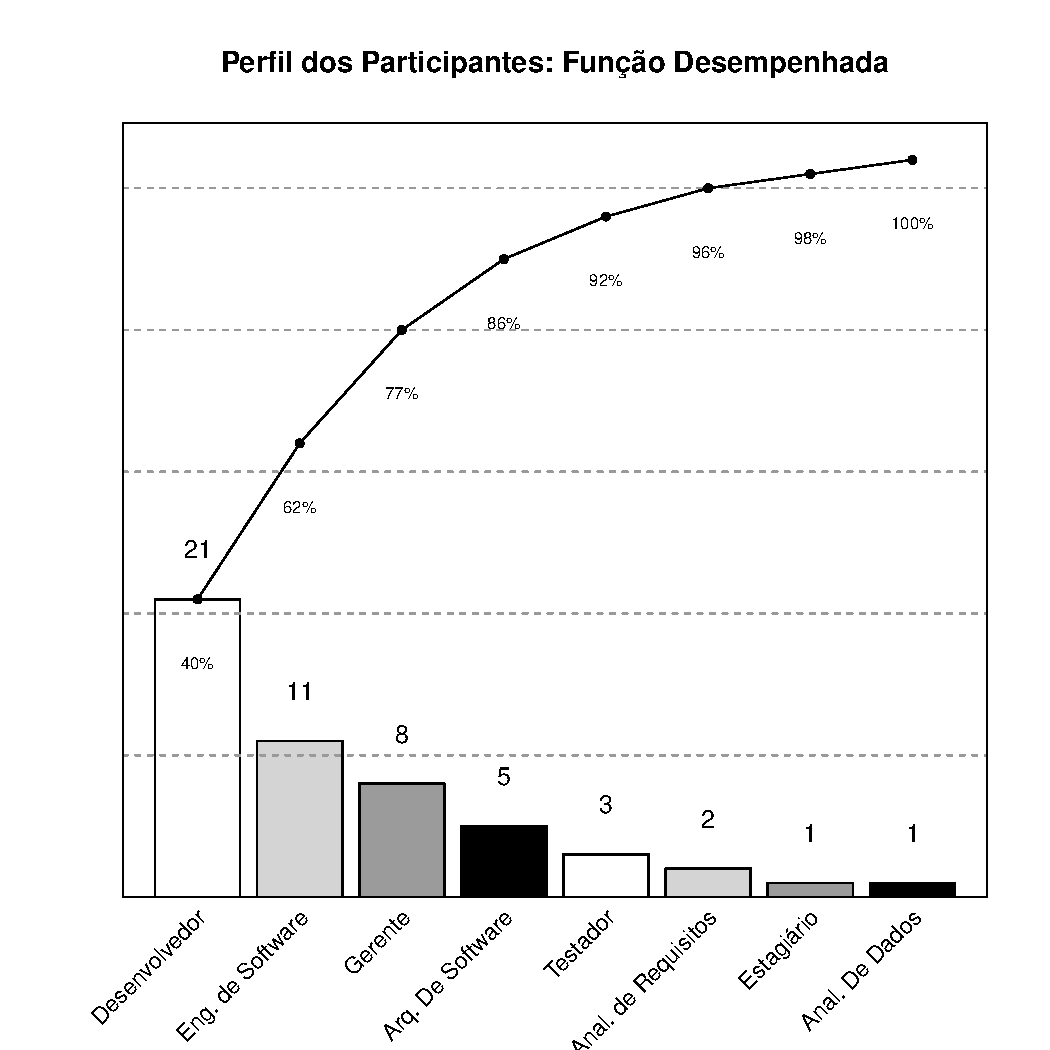
\includegraphics[width=0.8\linewidth]{./chapter-caracterizacao-ferramentas/img/grafico_escolha_ferramentas_funcao_participantes.pdf}
	\caption{Funções desempenhadas pelos participantes}
	\label{fig:grafico_escolha_ferramentas_funcao_participantes}
\end{figure}

O grupo de respondentes também incluem Engenheiros de Software, Gerentes de
Equipe e Arquitetos de Software que, junto com os Desenvolvedores, representam
mais de 80\% do total. Com relação a experiência verificamos que a maior parte
possui entre 3 e 10 anos, conforme pode ser verificado pela
Figura~\ref{fig:grafico_escolha_ferramentas_tempo_experiencia}.

\begin{figure}[htpb]
	\centering
	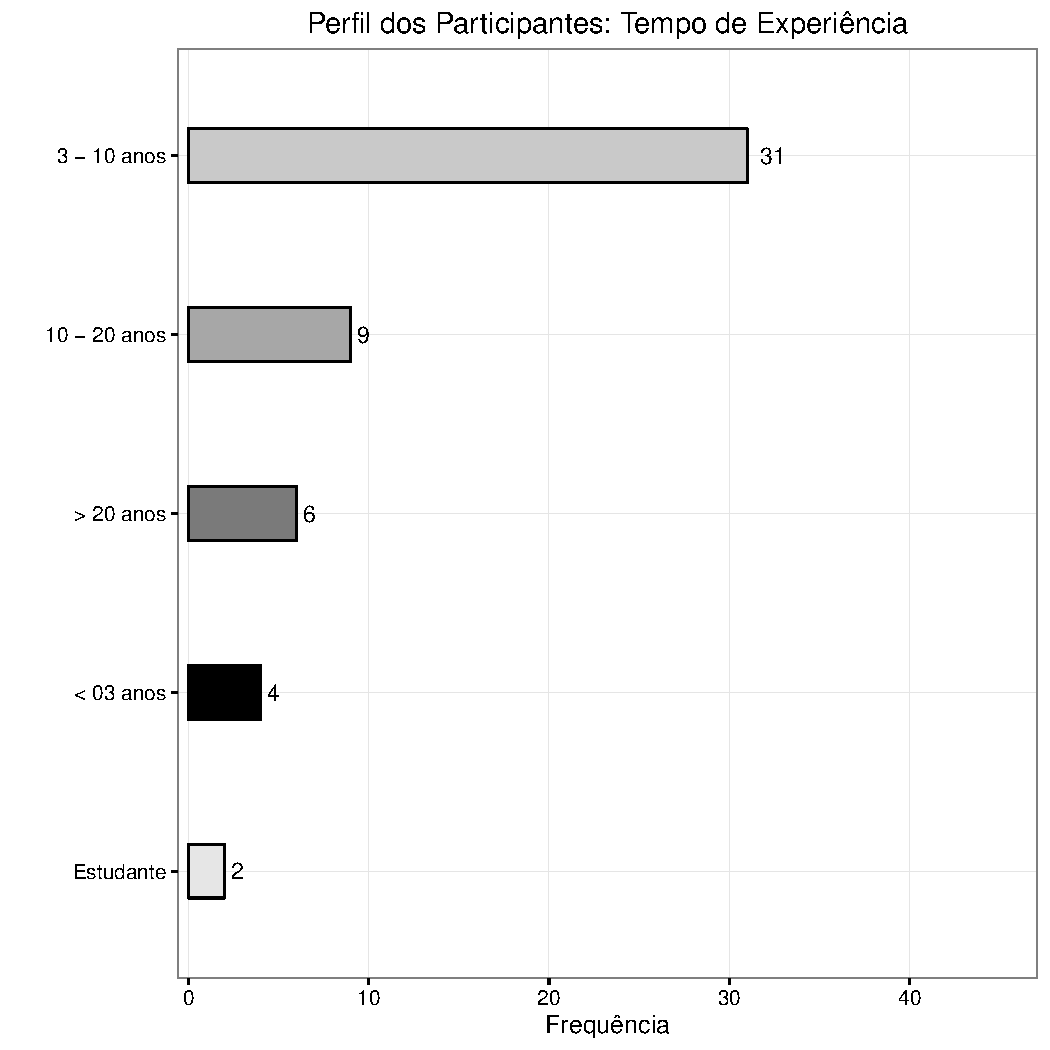
\includegraphics[width=0.8\linewidth]{./chapter-caracterizacao-ferramentas/img/grafico_escolha_ferramentas_tempo_experiencia.pdf}
	\caption{Tempo de Experiência}
	\label{fig:grafico_escolha_ferramentas_tempo_experiencia}
\end{figure}

Com relação ao tamanho da equipe em que os participantes fazem parte,
verificamos uma prevalência de entre equipe médias ( mais do que 10 membro) e
pequenas (2 a 5 membros). A
Figura~\ref{fig:grafico_escolha_ferramentas_tamanho_equipe} exibe o tamanho da
equipe dos participantes. Por sua vez, estas equipes estão predominantemente em
empresas privadas de software. Com relação ao local de trabalho verificamos
ainda que o segundo posto em número participantes ficou para empresas que
pertencem ao setor governamental. Esta distribuição pode ser visualizada na
Figura~\ref{fig:grafico_escolha_ferramentas_local_trabalho}.

\begin{figure}[htpb]
	\centering
	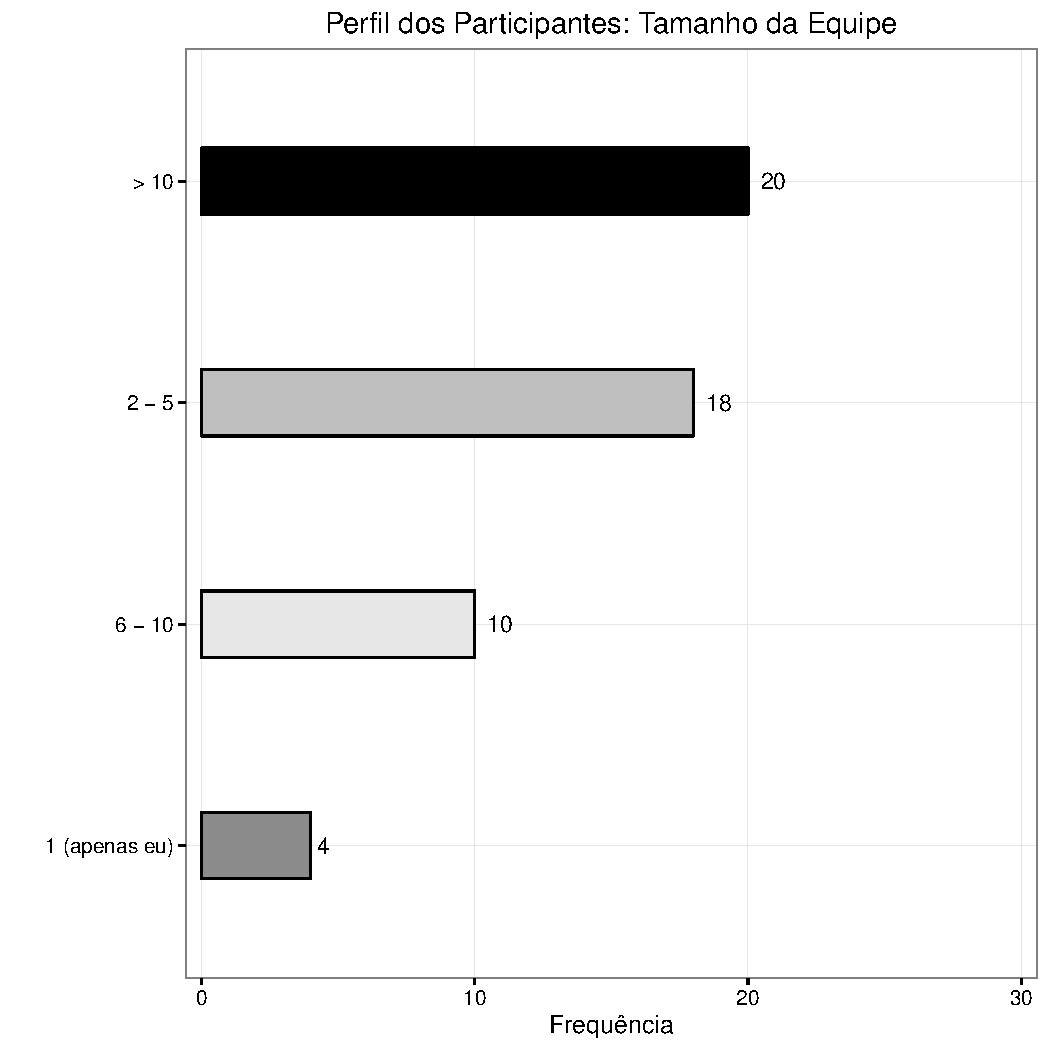
\includegraphics[width=0.8\linewidth]{./chapter-caracterizacao-ferramentas/img/grafico_escolha_ferramentas_tamanho_equipe.pdf}
	\caption{Tamanho da Equipe}
	\label{fig:grafico_escolha_ferramentas_tamanho_equipe}
\end{figure}

Em resumo o perfil do participantes se mostrou um desenvolvedor  entre três e
dez anos de experiência trabalhando em uma empresa privada de desenvolvimento de
software que com uma equipe de aproximadamente dez membros. Segundo o nosso
entendimento, como este perfil um profissional é capaz de nos ajudar a escolher
as ferramentas que estão disponíveis de modo a determinar a mais relevante. 

\begin{figure}[htpb]
	\centering
	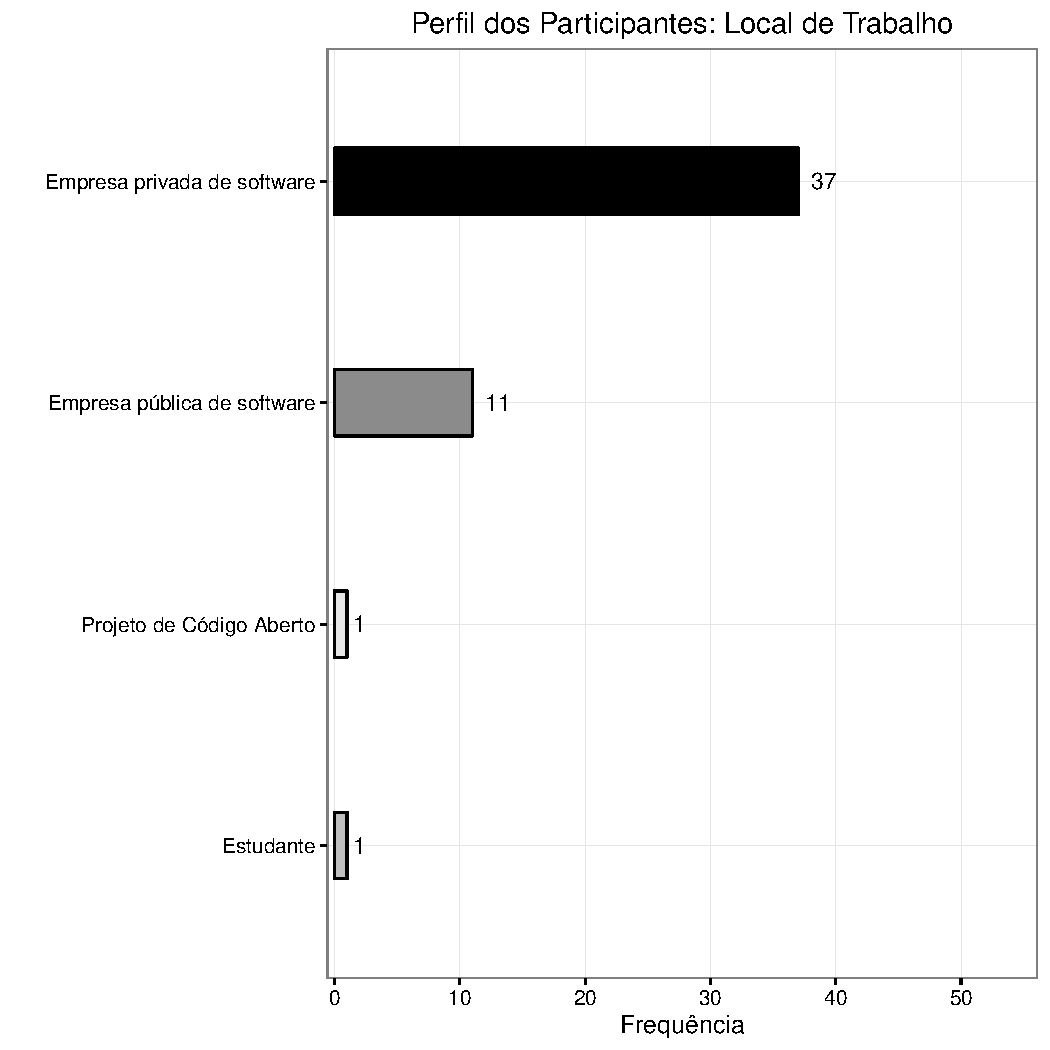
\includegraphics[width=0.8\linewidth]{./chapter-caracterizacao-ferramentas/img/grafico_escolha_ferramentas_local_trabalho.pdf}
	\caption{Local de trabalho}
	\label{fig:grafico_escolha_ferramentas_local_trabalho}
\end{figure}

\subsection{Ferramentas Escolhidas}
\label{subsec:resultados_ferramentas_escolhidas}

Utilizando a Equação~\ref{eq:escolha_ferramenta} obtivemos as ferramentas
apresentas na Tabela~\ref{tab:ferramenta_utilizadas_estudo}. Conforme pode ser
observado foi escolhida uma ferramenta para cada tipo de sistema. É importante
perceber ainda que as FGRM's \textit{Github e Gitlab} não estavam na lista
inicial de ferramentas, contudo, apareceram neste resultado final. Tal situação é
decorrente do fato de atribuímos o maior peso ($w_i = 5$) para aquelas
ferramentas que foram citadas pelos participantes em um campo próprio.  Neste
caso, devido a frequência que estas ferramentas foram lembradas pelos
profissionais elas acabaram por serem escolhidas. 

\begin{table}[htb]
\centering
\caption{Ferramentas utilizados no estudo}
\label{tab:ferramenta_utilizadas_estudo}
\resizebox{\textwidth}{!}{%
\begin{tabular}{|lccl|}
\hline
\multicolumn{1}{|c}{\textbf{Ferramenta}} & \textbf{Classificação} & \textbf{Versão} & \multicolumn{1}{c|}{\textbf{URL}}      \\ \hline
Bugzilla                                 & Ferramenta             & 5.0.3           & https://www.bugzilla.org               \\
Mantis Bug Tracker                       & Ferramenta             & 1.3.2           & https://www.mantisbt.org               \\
Redmine                                  & Ferramenta             & 3.3.1           & http://www.redmine.org/                \\
JIRA Software                            & Serviço                & 7.2.4           & https://br.atlassian.com/software/jira \\
Github Issue Tracking System             & Serviço                & \@-\@           & https://github.com/                    \\
Gitlab Issue Tracking System             & Serviço                & \@-\@           & https://gitlab.com/                    \\ \hline
\end{tabular}%
}
\end{table}


\subsection{Categorização das Ferramentas}
\label{subsec:categorizacao_ferramentas}

Após a inspeção da documentação e validação dos dados obtivemos um total de 123
cartões. Nós sistematizamos os cartões manualmente tendo em vista que não
existem ferramentas ou métodos capazes de automatizar o processo de construção
de hierarquias. Tendo em vista que nosso objetivo é derivar tópicos a partir do
conjunto inicial de cartões, optamos por realizar um \textit{ordenamento aberto}
dos cartões.  Naquele tipo de abordagem, os grupos são estabelecidos durante o
processo de Classificação os cartões em oposição a outra forma de utilização da
técnica onde a sistematização dos cartões ocorre com base em grupos
pré-determinados.  Ao final do processo obtivemos os seguintes tópicos listados
a seguir. Nas próximas seções apresentamos as funcionalidades que compõe cada um
deles.

\begin{enumerate}
	\item{Busca e Duplicados}
	\item{Extensão de Funcionalidades}
	\item{Gerenciamento da Informação}
	\item{Gerenciamento de Artefatos}
	\item{Internacionalização da Ferramenta}
	\item{Processo de Trabalho}
	\item{Segurança da Informação}
	\item{Suporte ao Trabalho do Desenvolvedor}
	\item{Triagem de RM's}
	\item{Visualização e Monitoramento de RM's}
\end{enumerate}

\subsubsection{Busca e Duplicados}

Este tópico foi criado para agrupar as funcionalidades relacionadas a busca de
RM's e a localização de duplicados.
\subsubsection{Extensão de Funcionalidades}

As funcionalidades que compõem este grupo têm por objetivo extensor o conjunto
de funcionalidades oferecidas através de uma arquitetura de plugins ou mediante
o suporte de
API's\footnote{\url{https://en.wikipedia.org/wiki/Application_programming_interface}}.
\subsubsection{Gerenciamento da Informação}

Este tópico contempla as funcionalidade que se dedicam ao armazenamento e
consistência das informações contidas na FGRM\@.

\subsubsection{Gerenciamento de Artefatos}

O processo de manutenção de software pode consumir ou gerar diversos artefatos,
tais como documentos de requisitos e arquiteturais dos software, código fonte,
registros (logs) de teste e assim por diante~\cite{cavalcanti2013bug}. Em alguns
contextos, devido ao volume de artefato gerados, é importante que a FGRM dê
suporte para armazenamento e recuperação deste ativos do processo de software.

\subsubsection{Internacionalização da Ferramenta}

Neste tópicos estão as características das FGRM que ajudam no desenvolvimento
e/ou adaptação de um produto, em geral softwares de computadores, para uma
língua e cultura de um país.

\subsubsection{Processo de Trabalho}
 Este ramo do esquema de classificação proposto foi criado para
 agrupar as funcionalidades que visão dar suporte ao processo de manter
 software.

\subsubsection{Segurança da Informação}

Neste grupo estão as características de uma FGRM que diretamente relacionada com
proteção de um conjunto de informações, no sentido de preservar o valor que
possuem para um indivíduo ou uma organização.

\subsubsection{Suporte ao Trabalho do Desenvolvedor}

Este tópico contém ideias sobre como o trabalho para desenvolvedores pode ser
reduzido, seja por melhor suporte de ferramentas (por exemplo, configuração
automática de espaços de trabalho) ou relatórios de bugs melhores com mais
dados.

\subsubsection{Triagem de RM's}

Este tópico descreve comentários sobre o processo de triagem de RM's. O processo
de atribuição de RM, também conhecido como triagem, possui como principal
objetivo encontrar o desenvolvedor mais capacitado para manipular uma dada RM\@.

\subsubsection{Visualização e Monitoramento de RM's}

Em diversos contextos, devido ao volume das RM's, é importante que as partes
interessadas na manutenção de software, possam visualizar e monitorar a situação
das requisições que estão analisadas em determinado período.

%\section{Discussão}
%\label{sec:discussao}

%Classificar envolve categorização, e há uma literatura sofisticada sobre
%categorização, taxonomia e semântica, todas as quais são potencialmente
%relevantes~\cite{rugg2005sorting}

%As técnicas de triagem são uma parte inestimável Engenheiro de conhecimento ou
%kit de ferramentas do engenheiro de requisitos.  Eles são simples de usar e
%combinam a flexibilidade de uso com um formalismo de representação altamente
%formalizado, preenchendo a lacuna entre as técnicas qualitativas e
%quantitativas.

\section{Ameças à Validade}
\label{sec:ameacas_a_validade}

Em grande parte dos estudos a generalidade dos resultados é muitas vezes
sacrificada pela riqueza e complexidade dos dados analisados. Neste sentido,
podemos afirmar que o processo de classificação é, por natureza, uma avaliação
subjetiva.

Uma ameaça à validade do trabalho está no processo de seleção das ferramentas.
Apesar da escolha ter sido realizada com suporte de profissionais envolvido em
manutenção de software, não podemos garantir que o número de respondentes pode
suportar que foi escolhido as ferramentas mais relevantes dentre aquelas
disponíveis. Neste mesmo sentido, a formula que foi utilizada para definir as
mais relevantes podem conter um enviesamentos sobretudo pela forma que os pesos
foram adotados, ou seja, não há como garantir que o fato de um participante
entender que uma determinada ferramenta é muito relevante ($w_j = 5$) mereça ser
ponderado cinco vezes mais que uma outra que não é conhecida ($w_j = 1$).
Todavia ao bem do nosso conhecimento não há técnicas para classificação que não
tenha influência da subjetividade.

Com relação à técnica de classificação utilizando Cartões de Ordenamento temos
dois pontos principais de ameaças aos resultados. Como a extração dos dados foi
realizada de forma manual pode ter ocorrido algum tipo de equívoco no processo
como por exemplo a  não coleta de determinada ferramenta por mero esquecimento.
Todavia, um número pequeno de ferramentas foi selecionada tendo em vista a
limitação desta extração manual. Um segundo ponto encontra-se na classificação
dos cartões. Apesar do processo ter sido realizado em pares pode ter ocorrido
uma classificação de forma incorreta o que pode acarretar em limitação dos
resultados apresentados. Esta situação pode ocorrer porque para algumas
funcionalidades não há uma fronteira clara para qual grupo ela pertence.

%\section{Resumo do Capítulo}
%\label{sec:resumo_do_capitulo}
